\subsection{Communication}

\indent 

\noindent\textbf{Communication ensure alignment between}:

\begin{itemize}
    \item Developers, testers, project managers
    \item Clients, users, external, stakeholders
\end{itemize}

\bigskip

\noindent\textbf{Types of Communication in IT projects}:

\begin{itemize}
    \item Written
    \item Verbal
    \item Presentation/Visual
    \item Non-verbal
\end{itemize}

\subsubsection{Communication in IT}

\indent 

IT Projects are collaborative and multidisciplinary.

\noindent\textbf{Communication in IT is critical for}:

\begin{itemize}
    \item Requirement Gathering
    \item Team Coordination
    \item Stakeholder Engagement
    \item Reporting Progress
\end{itemize}

\subsubsection{Written Communication}

\indent 

\noindent\textbf{Formal}:Emails, Reports, Contracts, Documentations, etc.

\noindent\textbf{Informal}: Slack chats, Shared Notes, etc.

\noindent\textbf{Best practices}: Be clear and concise; Avoid jargon unless necessary; Proofread before sending.

\subsubsection{Verbal Communication}

\indent 

Face-to-face, virtual meetings, stand-ups.

\noindent\textbf{Benefits}: Quick clarification, Builds trust.

\noindent\textbf{Skills needed}: Active listening, Speaking with clarity, Managing tone and pace.

\noindent\textbf{Pitfalls}: Dominance of few voices, missed follow-ups.

\subsubsection{Presentations}

\indent 

\noindent\textbf{Used for}: Project proposals, Stakeholder updates, Demos, etc.

\bigskip

\noindent\textbf{Key elements}:

\begin{itemize}
    \item Story telling (Problem $\Longrightarrow$ Solution $\Longrightarrow$ Impact)
    \item Visual Aids (Charts, Diagrams, Dashboards)
    \item Audience Awareness (Technical vs Non-technical)
\end{itemize}

\subsubsection{Effective Communication Frameworks}

\indent 

\noindent\textbf{7Cs of Communication}

\begin{itemize}
    \item \textbf{Clear}: Message should be easy to understand and avoid vague language
    \item \textbf{Concise}: Keep it short and to the point, avoid unnecessary details.
    \item \textbf{Concrete}: Use specific facts, data, or example rather than abstract statements.
    \item \textbf{Correct}: Ensure information is accurate and error free (grammar, spelling, etc.)
    \item \textbf{Coherent}: Message should be logical, well structured, and flow naturally.
    \item \textbf{Complete}: Provide all necessary information so there are no follow-up questions.
    \item \textbf{Courteous}: Be respectful, positive, and polite. Encourage collaboration.
\end{itemize}

\bigskip

\noindent\textbf{SBAR Framework}

\begin{itemize}
    \item \textbf{Situation}: State the immediate issue/problem clearly and briefly. What is happening right now?
    \item \textbf{Background}: Provide context or relevant history. What led to this issue? Why is it important?
    \item \textbf{Assessment}: Share your analysis or findings. What do you think is the cause? What is the impact?
    \item \textbf{Recommendation}: Propose next steps or actions to be taken. Clearly state what you need from the other person.
\end{itemize}

\subsubsection{Barriers to communication in IT Teams}

\begin{itemize}
    \item Technical jargon/acronyms
    \item Cultural and Language differences
    \item Remote collaboration challenges (time zones, etc.)
    \item Assumptions and lack of active listening
    \item Poor documentation >>> Knowledge gaps
\end{itemize}

\subsection{Teamwork}

\subsubsection{Importance of teamwork}

\indent 

IT projects are collaborative in nature.

Combines diverse expertise (developers, testers, designers, managers, 
business analysts)

\noindent\textbf{Teamwork leads to}:

\begin{itemize}
    \item Faster problem-solving
    \item Higher creativity \& innovation
    \item Shared responsibility \& accountability
    \item Stronger project outcomes
\end{itemize}

\bigskip 

\noindent\textbf{An effective IT Team}:

\begin{itemize}
    \item Clear roles \& responsibilities
    \item Trust \& psychological safety
    \item Open and respectful communication
    \item Shared goals and accountability
    \item Ability to adapt to change
    \item Balance of technical and soft skills
\end{itemize}

\subsubsection{Mistaken beliefs about teamwork}

\begin{itemize}
    \item “Teamwork means everyone has to agree” $\Longrightarrow$ \textbf{No, healthy disagreements drive better outcomes}
    \item “Teamwork slows things down” $\Longrightarrow$ \textbf{Actually, collaboration reduces rework and errors}
    \item “Good teams don’t have conflicts” $\Longrightarrow$ \textbf{Conflicts are normal; it’s how they’re resolved that matters}
    \item “Teamwork means equal contribution from all” $\Longrightarrow$ \textbf{Different roles contribute in different ways}
\end{itemize}

\subsubsection{Teamwork and Diversity}

\indent 

\noindent\textbf{Types of Diversity}:

\begin{itemize}
    \item Cultural and linguistic
    \item Educational and technical background
    \item Gender, age, and experiences
\end{itemize}

\bigskip

\noindent\textbf{Pros}: better problem-solving, user-centered products, broader perspectives, more innovation.

\noindent\textbf{Challenges}: communication barriers, unconscious bias.

\bigskip

\noindent\textbf{Team dynamics and Challenges}:

\begin{itemize}
    \item Unequal participation
    \item Dominant personalities vs quiet contributors
    \item Misaligned goals or unclear expectations
    \item Cross-cultural misunderstandings
    \item Remote/virtual team challenges (time zones, engagement)
\end{itemize}

\subsubsection{Belbin's Team Roles}

\indent 

\noindent\textbf{What are Belbin's Team roles?}

A framework developed by Dr. Meredith Belbin to identify nine behavioral roles 
people adopt in teams. Helps create balanced teams by ensuring all critical roles are covered. Roles are grouped into three categories: Social, Thinking, and Action/Task.

\bigskip

\noindent\textbf{Nine roles}:

\begin{itemize}
    \item \textbf{Social}: Resource Investigator, Team-worker, Coordinator
    \item \textbf{Thinking}: Plant, Monitor Evaluator, Specialist
    \item \textbf{Action/Task}: Shaper, Implementer, Completer Finisher
\end{itemize}

\bigskip

\noindent\textbf{Why does it matter?}

\begin{itemize}
    \item Encourages awareness of strengths and weaknesses.
    \item Prevents role overlap or gaps.
    \item Supports better teamwork and project outcomes.
\end{itemize}

\subsubsection{Psychological Safety – Google’s Project Aristotle}

\indent 

\noindent\textbf{What is Psychological safety?}

Shared belief that team members can take risks without fear of embarrassment 
or punishment. Encourages open communication, idea sharing, and learning from mistakes. Key driver of trust and collaboration in high-performing teams.

\bigskip

\noindent\textbf{Why it matters in IT projects?}

\begin{itemize}
    \item Promotes innovation and creativity.
    \item Reduces fear of speaking up about errors, leading to fewer failures.
    \item Improves engagement, morale, and resilience under pressure.
\end{itemize}

\bigskip

\noindent\textbf{How to create it?}

\begin{itemize}
    \item \textbf{Encourage curiosity}: Value questions and new ideas.
    \item \textbf{Normalize mistakes}: Treat errors as opportunities to learn.
    \item \textbf{Active listening}: Leaders and peers listen without judgment.
    \item \textbf{Inclusive environment}: Ensure all voices are heard, not just dominant ones.
    \item \textbf{Clear expectations}: Define roles, but allow flexibility for contributions.
\end{itemize}

\bigskip

\noindent\textbf{Impact on Teams}

\begin{itemize}
    \item Higher innovation and creativity.
    \item Faster problem-solving and adaptability.
    \item Stronger sense of belonging and collaboration
\end{itemize}

\subsubsection{Agile Teamwork Practices}

\begin{itemize}
    \item \textbf{Daily Standup}: Usually a daily meeting, lasting no more than 15 minutes. Team members describe what they worked in the previous day, and what are they intend to work on today. It should not be detailed.
    \item \textbf{Sprint Planning}: The team uses this meeting to decide what to do during the sprint.
    \item \textbf{Sprint Review}: At the end of a sprint or milestone, the team reviews their accomplishments against the planned sprint work. The team will often use this meeting to demonstrate the results of their work and get feedback from stakeholders.
    \item \textbf{Sprint Retrospective}: At the end of an iteration, the team discusses what worked well, and what could be improved.
\end{itemize}

\subsubsection{Conflicts in the Workplace}

\indent 

\noindent\textbf{Common Sources}

\begin{itemize}
    \item Competing priorities
    \item Miscommunication
    \item Personality clashes
    \item Ambiguous responsibilities
    \item Resource constraints
\end{itemize}

\bigskip

\noindent\textbf{Impact if unmanaged}

\begin{itemize}
    \item Reduced productivity
    \item Low morale
    \item Stakeholder dissatisfaction
\end{itemize}

\subsubsection{Task Conflict VS Relationship Conflict}

\indent 

\noindent\textbf{Task conflict (Cognitive conflict)}

\begin{itemize}
    \item Disagreements about \textbf{work-related issues} (goals, ideas, processes, tasks).
    \item Can be constructive, stimulates critical thinking, innovation, and better decisions.
\end{itemize}

\bigskip

\noindent\textbf{Relationship conflict (Affective conflict)}

\begin{itemize}
    \item Based on \textbf{personal incompatibilities} (personality clashes, tension, mistrust).
    \item Usually \textbf{destructive}, reduces team cohesion, satisfaction, and performance.
\end{itemize}

\subsection{Stakeholder Management}

\indent

\noindent\textbf{Who are stakeholders?}

Individuals, groups, or organizations affected by or having an interest in the project.

\bigskip

\noindent\textbf{Why does stakeholder management matter?}

\begin{itemize}
    \item Aligns expectations with deliverables
    \item Minimizes conflict and scope creep
    \item Builds trust and project credibility
\end{itemize}

\subsubsection{Stakeholder analysis and mapping}

\indent 

The main purpose of this step is to understand stakeholder needs, interests, and influence.

\noindent\textbf{The major steps for stakeholder analysis and mapping are}:

\begin{itemize}
    \item Identify stakeholders (internal \& external)
    \item Assess their interests, expectations, and influence
    \item Prioritize based on their importance
    \item Develop tailored engagement strategies
\end{itemize}

\bigskip

\noindent\textbf{Power Interest Matrix}: This is a tool to categorize the 
stakeholders by Power (ability to influence the project) \& Interest (level of concern or involvement). Helps decide how much time and effort to invest in managing each stakeholder.

\begin{figure}[h]
    \centering
    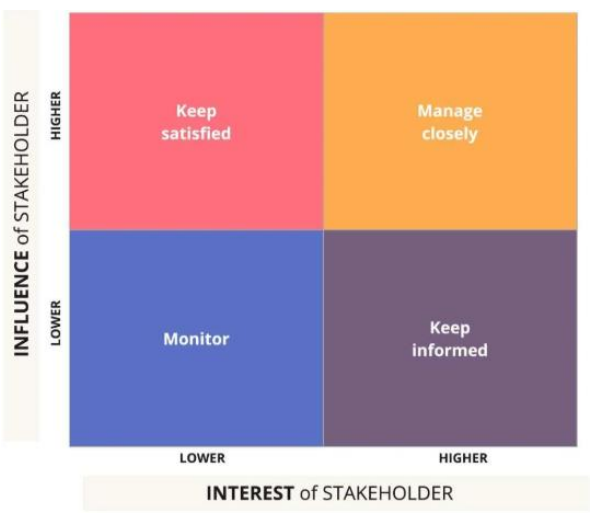
\includegraphics[width=0.5\linewidth]{figures/Week 4/Power Interest Matrix.png}
\end{figure}

\bigskip

\noindent\textbf{Salience Model}: An advanced stakeholder analysis tool. Categorises stakeholders based on 3 attributes: Power (ability to influence), Legitimacy: (appropriateness of their involvement), Urgency (how quickly they require attention)

\begin{figure}[h]
    \centering
    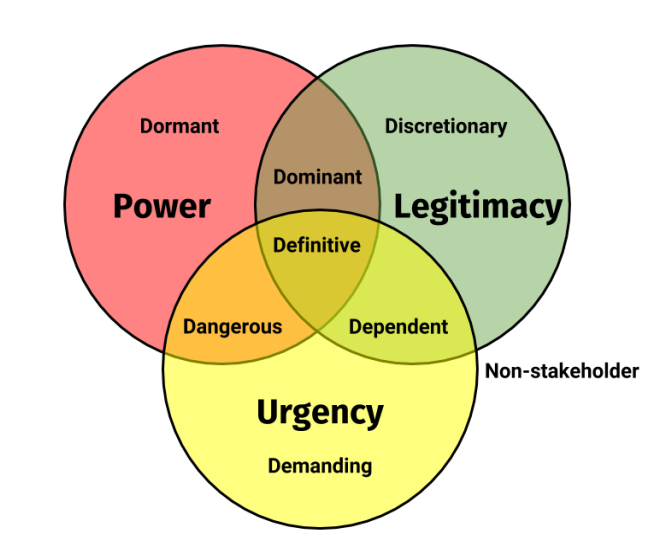
\includegraphics[width=0.5\linewidth]{figures/Week 4/Salience Model.png}
\end{figure}

\begin{itemize}
    \item \textbf{Definitive (Power + Legitimacy + Urgency)}: Highest priority
    \item \textbf{Dominant (Power + Legitimacy)}: Strong influence, need active management
    \item \textbf{Dependent (Legitimacy + Urgency)}: Need support to gain power (e.g., end-users)
    \item \textbf{Dangerous (Power + Urgency)}: Can disrupt if ignored
    \item \textbf{Dormant (Power only)}: Potential influence if mobilized
    \item \textbf{Discretionary (Legitimacy only)}: Low involvement, can support reputation
    \item \textbf{Demanding (Urgency only)}: Attention-seeking, but low impact
\end{itemize}

\subsubsection{Engagement strategies}

\indent 

One must match the strategy to the stakeholder category. There are several levels of engagement:

\begin{itemize}
    \item \textbf{Inform}: Low power, low interest → newsletters, emails
    \item \textbf{Consult}: Seek input from those affected
    \item \textbf{Involve}: Engage in workshops, feedback sessions
    \item \textbf{Collaborate}: Co-create solutions, joint decision-making
    \item \textbf{Empower}: Give decision-making authority (e.g., product owners in Agile)
\end{itemize}

Use multiple channels: reports, demos, townhalls, dashboards.

\subsubsection{Challenges in Stakeholder Management}

\begin{itemize}
    \item Changing requirements during project lifecycle
    \item Conflicting interests between stakeholder groups
    \item Cultural/language barriers (global IT teams)
    \item Stakeholders with unrealistic expectations
    \item Hidden stakeholders not identified early
    \item Over- or under-communicating with certain groups
\end{itemize}

\subsubsection{Best practices}

\begin{itemize}
    \item Start stakeholder analysis \textbf{early} and update regularly
    \item Use \textbf{clear communication frameworks} (7Cs, SBAR)
    \item Manage expectations $\Longrightarrow$ under-promise, over-deliver
    \item Foster \textbf{trust and transparency}
    \item Document decisions \& agreements
    \item Balance time spent across stakeholder groups (don’t neglect “low power, high interest” users)
    \item Regular engagement $\Longrightarrow$ reviews, feedback loops, demos
\end{itemize}

\subsection{How does it all come together?}

\indent 

\noindent\textbf{Interconnected nature}:

\begin{itemize}
    \item Communication is the \textbf{glue}: ensures clarity between team members and stakeholders.
    \item Teamwork is the \textbf{engine}: drives collaboration, innovation, and delivery.
    \item Stakeholder Management is the \textbf{direction}: ensures the team is building the right thing, aligned with expectations.
\end{itemize}

\bigskip

\noindent\textbf{Why can't each of these 3 work in isolation?}

\begin{itemize}
    \item Poor communication $\Longrightarrow$ teamwork suffers, stakeholders lose trust.
    \item Poor teamwork $\Longrightarrow$ communication breaks down, deliverables slip.
    \item Poor stakeholder management $\Longrightarrow$ even a strong team delivering great work risks rejection if it doesn’t meet stakeholder needs.
\end{itemize}

\subsection{Question}

\subsubsection{End of Lecture Questions}

\begin{itemize}
    \item What are the 7 Cs of Communication, and why are they important in IT projects?
    \item According to Tuckman’s model, what typically happens during the “Storming” stage of team development?
    \item What are some conflict resolution strategies, and when might you use them?
    \item What are two common challenges in stakeholder management, and how can they be addressed?
    \item Compare the Power–Interest Matrix and the Salience Model. How do they differ in analyzing stakeholders?
    \item How do communication, teamwork, and stakeholder management work together to ensure IT project success?
\end{itemize}

\subsubsection{Case Study}

\indent

A software company is developing a mobile banking app for a major bank.

\noindent\textbf{Stakeholders}: The bank’s executives (sponsors), compliance officers (regulators), customer support staff, IT developers, and end-users (customers).

\noindent\textbf{Situation}:

\begin{itemize}
    \item During development, developers find conflicting requirements from executives (wanting faster release) and compliance officers (demanding more security checks).
    \item The team also faces internal conflict: testers complain that developers don’t provide enough documentation, while developers argue that deadlines are too tight.
    \item The client complains about unclear updates, saying they’re “not sure what’s really happening with the project.”
\end{itemize}

\bigskip

\noindent\textbf{Question}:

\begin{itemize}
    \item Identify at least two communication failures in this scenario.
    \item Which stage of Tuckman’s model does this team appear to be in? Why?
    \item What conflict resolution strategy would you apply between developers and testers?
    \item Place the executives, compliance officers, and end-users into the Power–Interest Matrix.
    \item How can better communication, teamwork, and stakeholder management together prevent project delays in this scenario?
\end{itemize}